\chapter{Subsistema de recolección y envío}

\section{Arquitectura del subsistema}
El subsistema de recolección y envío está formado por dos módulos, los cuales actúan en el dispositivo ubicuo. Esta es una división a nivel lógico y existe para reducir a problemas más simples el problema general, aunque nada impide que una herramienta implemente dos módulos.

%%Figura de la arquitectura

\subsection{Módulo de recolección}
El módulo de recolección es el encargado de recoger los eventos en el dispositivo ubicuo, para que luego el módulo de envío pueda consumirlos. 
\\\\
En concreto para este proyecto los eventos que se recogen son logs y crashlogs. Los logs servirán para llevar a cabo la monitorización y los crashlogs el seguimiento de errores.
\\\\
Para generar logs se han de explicitar en el código ahí donde el programador considere adecuado, los crashlogs se generan automáticamente cuando la aplicación termina inesperadamente.
\\\\
Los logs se recolectan en tiempo de ejecución y se almacenan en el dispositivo ubicuo para que el módulo de envío los consuma cuando sea pertinente.
\\\\
Los crashlogs se recolectan cuando la aplicación termina inesperadamente y no se almacenan en el dispositivo, sino que de forma inmediata el módulo de envío los consume. Se ha decidido que no se almacenen en el dispositivo puesto que, se considera que tienen más prioridad que los logs, y porque no se puede asegurar que se lleguen a almacenar en el dispositivo o que la aplicación pueda volverse a abrir después de que el crash haya sucedido. Así pues se invoca directamente al módulo de envío para que consuma tal crashlog.

\subsection{Módulo de envío}
El módulo de envío es el encargado de consumir los eventos que ha recolectado el módulo de recolección y enviar tales eventos al módulo de recepción del subsistema de recepción e ingesta.
\\\\
El envío de los logs lo hace cuando la aplicación se cierra correctamente. Es entonces cuando consume los logs almacenados en el dispositivo y los envía al módulo de recepción.
\\\\
El envío de los crashlogs lo hace cuando la aplicación se ha cerrado inesperadamente. Es entonces cuando consume el crash generado y lo envía al módulo de recepción.

\section{Estructura del sistema}

\subsection{Módulo de recolección}
El módulo de recolección está integrado por dos librerías. Una librería se encarga de recolectar los logs y otra los crashlogs.
\\\\
La librería encargada de recolectar logs como mínimo ha de permitir que el programador defina logs en el punto del programa donde este considere oportuno, y que se pueda definir el destino de los logs.

La librería encargada de recolectar crashlogs como mínimo ha de identificar cuando se ha producido un cierre inesperado de la aplicación, recuperar el error que ha notificado el sistema sobre el cierre inesperado, formar un crashlog con la información recopilada y permitir definir el destino del crashlog.

\subsection{Módulo de envío}
El módulo de envío está integrado por una librería. Esta librería se encarga de enviar los logs y los crashlogs recolectados mediantes peticiones HTTP. Como mínimo esta librería ha de poder formar una petición HTTP conteniendo los eventos recolectados, y enviarla a un destino.

\section{Herramientas utilizadas}

Las herramientas utilizadas para llevar a cabo los módulos han sido librerías para Android.

\subsection{Módulo de recolección}
Para llevar a cabo la recolección de logs se ha utilizado la librería Logback\cite{Tfg:logbackandroid} en su versión para Android. Esta librería permite definir en que punto del programa se quiere generar un log y redirigir la salida del log a diferentes destinos. Esta librería también nos permite editar el formato de salida del log así como la metainformación que se añade al log.

Para llevar a cabo la recolección de crashlogs se ha utilizado la librería ACRA\cite{Tfg:acra}. Esta librería detecta cuando una aplicación ha acabado inesperadamente y genera un crashlog con información de valor para reconocer que puede haber pasado. Esta librería también permite redirigir la salida del crashlog a diferentes destinos, editar el formato de salida del crashlog y la metainformación que se añade al crashlog.

\subsection{Módulo de envío}
Para llevar a cabo el envío de logs y crashlogs se ha utilizado la librería OkHttp\cite{Tfg:okhttp} que permite hacer peticiones HTTP\cite{Tfg:HTTPv1-1}. Se ha escogido esta librería por la rapidez con la que se puede programar lo que se desea para este proyecto, a parte del uso eficiente que hace de los recursos del sistema.

\section{Configuración del subsistema}

\subsection{Módulo de recolección}


Del módulo de recolección se han configurado los siguientes factores:

\subsubsection{Metadatos}
Metadatos hace referencia a toda la información que se recolecta a parte de la información de valor del evento. La información de valor n el caso de los logs es el mensaje de define el programador, en el caso de los crashlogs es el mensaje de error del crash.

De los los logs se recogen metadatos porque se consideran útiles para entender el contexto del log, los metadatos que se recogen son:

\begin{itemize}	
	\item \textbf{Hora del evento}: Hora en la que se produce el evento
	\item \textbf{Tiempo que transcurre desde que se inició la aplicación}: Una resta entre la hora que se produce el evento y la hora que se inició la aplicación.
	\item \textbf{Nivel}: Los logs pueden tener varios niveles, nivel informativo, de debug, de error, y más niveles que se pueden definir.
	\item \textbf{Nombre del thread}: Nombre del thread que lanza el log para que sea recolectado.
\end{itemize}

De los los crashlogs se recogen metadatos porque se consideran útiles para entender el contexto del crashlog y poder solucionar el error cuanto antes, los metadatos que se recogen son:

\begin{itemize}
	\item Versión de la aplicación
	\item Modelo del dispositivo
	\item RAM total del dispositivo
	\item RAM disponible en el momento del crash
	\item Versión de Android
	\item Tipo de CPU
	\item Tipos de CPU soportadas por el dispositivo
\end{itemize}

\subsubsection{Formato}
El formato escogido para representar tanto logs, como crashlogs ha sido un objeto JSON puesto que nos aporta el poder tratar el evento de manera fácil y para cumplir con los requisitos de formato que exige el módulo de recepción. Cada dato que se quiere incluir en el evento es un par clave-valor, donde la clave es fija y el valor depende del estado del dispositivo. Las claves de los crahslogs no se han podido definir, sino que ACRA define las que han de ser. En el caso de los logs sí que se han podido definir, para reducir el uso de red y de almacenamiento estas claves son tan solo un carácter, el módulo de transformación se configurará para que sea capaz de enriquecer los logs y de reconocer que significa cada carácter. 

\subsubsection{Destino}
Destino hace referencia a donde se envían los eventos una vez se han recolectado. 
Los logs no pasan directamente al módulo de envío, sino que se almacenan en un archivo de texto en el dispositivo ubicuo para que cuando la aplicación se cierre, el módulo de envío los consuma de ese archivo.
Los crashlogs pasan directamente a disposición del módulo de envío una vez se recolectan. No se almacenan en persistencia. 

\subsection{Módulo de envío}

Del módulo de envío se han configurado los siguiente factores:

\begin{itemize}
	\item \textbf{Cuándo se hace el envío}: En el caso de los logs, el envío se hace una vez la aplicación se ha cerrado, se hace así para no interferir en el uso de red mientras la aplicación está corriendo. En Android es posible detectar cuando se va a cerrar una aplicación y ejecutar código. \\ En el caso de los crashlogs el envío se hace justo cuando el crash sucede, se hace así ya que nada asegura que la aplicación pueda volverse a abrir después de que un crash haya sucedido. La librería ACRA nos permite llevar a cabo este comportamiento con los crashlogs.
	
	\item \textbf{Destino}: El destino tanto de los logs como de los crashlogs es el módulo de recepción, por lo que se ha configurado para que sean enviados ahí. Dentro del módulo de ingesta, logs y crashlogs van a destinos lógicos diferentes, por lo que también se ha configurado su destino dentro del módulo de ingesta.
	
	\item \textbf{Cómo se hace el envío}: En el caso de crashlogs no hay más opción a que cada petición HTTP POST hacía el módulo de recepción contenga tan solo un crashlog. En el caso de los logs se puede enviar una petición HTTP POST por cada log o envíar una petición HTTP POST con todos los logs recolectados durante la sesión. Se ha escogido enviar una sola petición HTTP POST con todos los logs recolectados para no saturar al módulo de recepción atendiendo peticiones.
\end{itemize}

\subsection{Vista general del subsistema}
En la figura \ref{fig:subrecenv} se puede ver como se relacionan los módulos y las herramientas del subsistema. Las flechas indican el sentido del flujo de datos.

\begin{figure}
	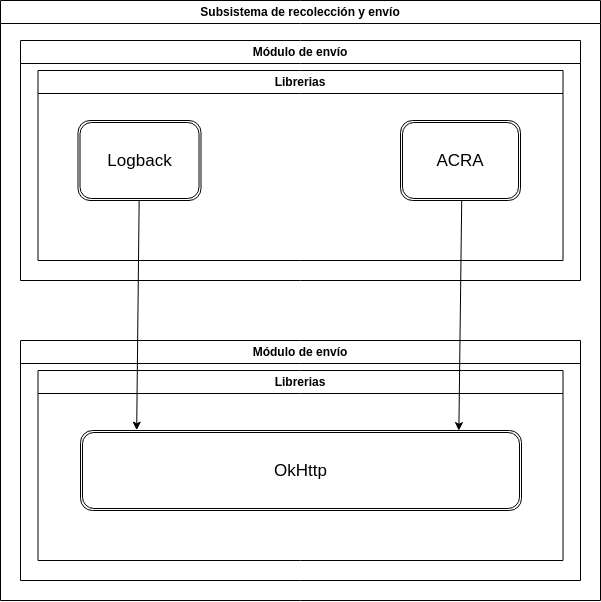
\includegraphics[width=\linewidth]{Moduloss-subrecenv.png}
	\caption{Vista general del subsistema de recolección y envío}
	\label{fig:subrecenv}
\end{figure}













